\section{gyakorlat (2025. november 19.)}
\subsection{}

TODO óra eleje

$6 \cdot 6  \cdot 6 \cdot 6 \cdot 6 \cdots 6$ 
TODO underbrace-es rész

Hogyan lehet ezt felgyorsítani?

$6^{1589} \rightarrow$ kitevő kettes számrendszerben


1589 : 2 = 794
 18
  09
   1

794 : 2 = 397
19
14
0

397 : 2 = 198
 19
  17
   1

198 : 2 = 99
 18
  0

99 : 2 = 49
19
 1
  
49 :  2 = 24
09
 1

24 : 2 = 12
04
 0

12 : 2 =6
 0

6 : 2 = 3
0

3 : 2 = 1
1

1 : 2 = 0
1



1 1 0 0 0 1 1 0 1 0 1
1024 512 256 128 64 32 16 8 4 2 1

1024 + 512 + 32 + 16 + 4 + 1 = 1589 (ahol 1-esek vannak)


Észrevétel: $\mathcal{O}(\log \text{kitevő})$ "elemi" művelet a kette számrendszerre átírás

Ezek után jön a piszkos trükk:
$6^{1589} = 6^{1024 + 512 + 32 + 16 + 4 + 1} = 6^{1024} \cdot 6^{512} \cdot 6^{32} \cdot 6^{16} \cdot 6^{4} \cdot 6^{1}$
TODO??
$6 mod 31 = 6$

$6^2 mod 31 = 5$

$6^4 = (6^2)^2 mod 31 = 5^2 mod 31 = 25 mod 31 = 25$

$6^8 = (6^4)^2 mod 31 = 25^2 mod 31 = 225 mod 31 = 8$

$6^16 = (6^8)^2 mod 31 = 8^2 mod 31 = 64 mod 31 = 2$ DONE

$6^32 = (6^16)^2 mod 31 = 2^2 mod 31 = 4$ DONE 

TODO
$6^64 = (6^32)^2 mod 31 = 4^2 mod 31 = 16$

$6^128 = (6^64)^2 mod 31 = 8^2 mod 31 = 64 mod 31 = 2$

$6^256 = (6^128)^2 mod 31 = 8^2 mod 31 = 64 mod 31 = 2$
TODO

$6^512 = (6^256)^2 mod 31 = 2^2 mod 31 = 4$ DONE

$6^1024 = (6^512)^2 mod 31 = 4^2 mod 31 = 16$ DONE

Így $6^{1024} \cdot 6^{512} \cdot 6^{32} \cdot 6^{16} \cdot 6^{4} \cdot 6^{1} mod 31$
$16 \cdot 4 \cdot 4 \cdot 2 \cdot 25 \cdot 6 mod 31$
TODO underbrace

16 * 25 = 400 -> 28

28 * 6 = 168 -> 13

=> $6^{1589} \equiv 13 mod 31$
TODO

13: ennyi a maradék a 31-gyel osztásnál

TODO

-re csökkent

Mi ennek a jelentősége?

Kitevő, mint input mérete O(log kitevő)

Ehhez képest \Theta(kitevő) exponenciálisan nagyobb

Így a naiv algoritmus exponenciális a bemenet méretében.
A piszkos  trükk ezt viszi le lineárisra (a bemenet méretében)

Előadásra visszatérve
$a_1, a_2, \cdots, a_n \longrightarrow B$

Részhalmaz-összeg: mindenkit egyszer használhatunk
Pénzváltás: többször is.
Nyilván
$a_1$-et max $\left\lfloor \frac{B}{a_1} \right\rfloor$,
$a_2$-t max $\left\lfloor \frac{B}{a_2} \right\rfloor$
$\vdots$
alkalommal


Pénzváltás naiv visszavezetése a részhalmaz-összegre:

$\underbrace{a_1, \cdots, a_1}_{\%TODO}, \underbrace{a_2, \cdots, a_2}_{\%TODO}, \cdots, \underbrace{a_n, \cdots, a_n}_{\%TODO} \rightarrow B$

Probléma: az input mérete a bemenet méretében, különös tekintettel B-re exponenciálisan nagy lett.

Nyilván azok az $a_i$-k, amelyek nagyobban $B$-nél nem sok vizet zavarnak, így a bemenet mérete $\mathcal{O}(n \log B)$ (nagyon precízen $\mathcal{O}((n + 1) \log B)$) a részhalmaz-összegnél.

Ha most $n$ lineáris $B$-ben, akkor ez $B \cdot \log B$ nagyságrendű, ami $2^{\log_2 B} \cdot B$, és ez exponenciálisan nagy $B$ méretében.

Ez azt jelenti, hogy hiába is lenne mondjuk egy kvadratikus algoritmusunk a részhalmaz-összegre (senki nem ismer ilyet), az exponenciális ideig futna a pénzváltásból előállított inputon.

A piszkos trükk itt:
$\underbrace{a_1, \cdots, a_1}_{\left\lfloor \frac{B}{a_1} \right\rfloor} \rightarrow$ amit ezekből elő tudunk állítani összegként, azt mind elő tudjuk állítani sokkal kevesebb számból is: $a_1, 2 a_1, 4 a_1, 8 a_1, \cdots, 2^{\left\lfloor \log_2 B \right\rfloor} a_1$
Ezzel a $\left\lfloor \frac{B}{a_1} \right\rfloor$ db szám lecsökken $\left\lfloor \log_2 B \right\rfloor$ darabra.

Így a transzformált bemenet mérete már nem exponenciális $\log B$-hez képest (igazából lineáris)!



\textbf{Példa} \hl{(zh. feladat)}:\\
Kitöltés menete:
TODO
\begin{itemize}
    \item Ha megegyeznek: átlósan átvesszük
    \item Ha különbözőek: 
\end{itemize}

minimális értéket akarjuk átvenni

megállapodás: "óramutató járásával ellentétesen" (egyenlőségkor elsősorban felülről, aztán átlóból, majd vízszintesen)

átlós út: lecseréljük az egyik betűt a másikra
függőleges út: beszúrom a másik betűt, törlöm az elsőt
az átlós út hatékonyabb, mint a függőleges út

\begin{tabular}{cccccccccccccc}
  &                                                  &                         & B                                              & A                                                                & A                                                                & C                                                                & B                                                                 & B                                                                 & A                                                                 & A                                                                 & C                                                                 & B                                                                 & C                                                                 \\
  &                                                  & 0                       & 1                                              & \fcolorbox{blue}{white}{2}                                       & \fcolorbox{blue}{white}{3}                                       & \fcolorbox{blue}{white}{4}                                       & 5                                                                 & \fcolorbox{blue}{white}{6}                                        & \fcolorbox{blue}{white}{7}                                        & \fcolorbox{blue}{white}{8}                                        & \fcolorbox{blue}{white}{9}                                        & \fcolorbox{blue}{white}{10}                                       & \fcolorbox{blue}{white}{11}                                       \\ \cline{3-14} 
  & \multicolumn{1}{l|}{0}                           & \multicolumn{1}{l|}{0}  & \multicolumn{1}{l|}{\cellcolor[HTML]{34CDF9}3} & \multicolumn{1}{l|}{6}                                           & \multicolumn{1}{l|}{9}                                           & \multicolumn{1}{l|}{12}                                          & \multicolumn{1}{l|}{15}                                           & \multicolumn{1}{l|}{18}                                           & \multicolumn{1}{l|}{21}                                           & \multicolumn{1}{l|}{24}                                           & \multicolumn{1}{l|}{27}                                           & \multicolumn{1}{l|}{30}                                           & \multicolumn{1}{l|}{33}                                           \\ \cline{3-14} 
A & \multicolumn{1}{l|}{\fcolorbox{blue}{white}{1}}  & \multicolumn{1}{l|}{3}  & \multicolumn{1}{l|}{\angledarrow{135} 5}       & \multicolumn{1}{l|}{\cellcolor[HTML]{34CDF9}\angledarrow{135} 3} & \multicolumn{1}{l|}{\angledarrow{135} 6}                         & \multicolumn{1}{l|}{\angledarrow{180} 9}                         & \multicolumn{1}{l|}{\angledarrow{180} 9}                          & \multicolumn{1}{l|}{\angledarrow{180} 15}                         & \multicolumn{1}{l|}{\angledarrow{135} 18}                         & \multicolumn{1}{l|}{\angledarrow{135} 21}                         & \multicolumn{1}{l|}{\angledarrow{180} 24}                         & \multicolumn{1}{l|}{\angledarrow{180} 27}                         & \multicolumn{1}{l|}{\angledarrow{180} 30}                         \\ \cline{3-14} 
B & \multicolumn{1}{l|}{\fcolorbox{blue}{white}{2}}  & \multicolumn{1}{l|}{6}  & \multicolumn{1}{l|}{\angledarrow{135} 3}       & \multicolumn{1}{l|}{\angledarrow{90} 6}                          & \multicolumn{1}{l|}{\cellcolor[HTML]{34CDF9}\angledarrow{135} 8} & \multicolumn{1}{l|}{\angledarrow{135} 11}                        & \multicolumn{1}{l|}{\angledarrow{135} 9}                          & \multicolumn{1}{l|}{\angledarrow{135} 12}                         & \multicolumn{1}{l|}{\angledarrow{180} 15}                         & \multicolumn{1}{l|}{\angledarrow{180} 18}                         & \multicolumn{1}{l|}{\angledarrow{180} 21}                         & \multicolumn{1}{l|}{\angledarrow{135} 24}                         & \multicolumn{1}{l|}{\angledarrow{180} 27}                         \\ \cline{3-14} 
C & \multicolumn{1}{l|}{\fcolorbox{blue}{white}{3}}  & \multicolumn{1}{l|}{9}  & \multicolumn{1}{l|}{\angledarrow{90} 6}        & \multicolumn{1}{l|}{\angledarrow{135} 8}                         & \multicolumn{1}{l|}{\angledarrow{90} 11}                         & \multicolumn{1}{l|}{\cellcolor[HTML]{34CDF9}\angledarrow{135} 8} & \multicolumn{1}{l|}{\cellcolor[HTML]{34CDF9}\angledarrow{180} 11} & \multicolumn{1}{l|}{\angledarrow{135} 14}                         & \multicolumn{1}{l|}{\angledarrow{135} 17}                         & \multicolumn{1}{l|}{\angledarrow{135} 20}                         & \multicolumn{1}{l|}{\angledarrow{135} 18}                         & \multicolumn{1}{l|}{\angledarrow{180} 21}                         & \multicolumn{1}{l|}{\angledarrow{135} 24}                         \\ \cline{3-14} 
B & \multicolumn{1}{l|}{\fcolorbox{blue}{white}{4}}  & \multicolumn{1}{l|}{12} & \multicolumn{1}{l|}{\angledarrow{90} 9}        & \multicolumn{1}{l|}{\angledarrow{90} 11}                         & \multicolumn{1}{l|}{\angledarrow{135} 13}                        & \multicolumn{1}{l|}{\angledarrow{90} 11}                         & \multicolumn{1}{l|}{\angledarrow{135} 8}                          & \multicolumn{1}{l|}{\cellcolor[HTML]{34CDF9}\angledarrow{135} 11} & \multicolumn{1}{l|}{\angledarrow{180} 14}                         & \multicolumn{1}{l|}{\angledarrow{180} 17}                         & \multicolumn{1}{l|}{\angledarrow{180} 20}                         & \multicolumn{1}{l|}{\angledarrow{135} 18}                         & \multicolumn{1}{l|}{\angledarrow{180} 21}                         \\ \cline{3-14} 
C & \multicolumn{1}{l|}{\fcolorbox{blue}{white}{5}}  & \multicolumn{1}{l|}{15} & \multicolumn{1}{l|}{\angledarrow{90} 12}       & \multicolumn{1}{l|}{\angledarrow{90} 14}                         & \multicolumn{1}{l|}{\angledarrow{90} 16}                         & \multicolumn{1}{l|}{\angledarrow{135} 13}                        & \multicolumn{1}{l|}{\angledarrow{90} 11}                          & \multicolumn{1}{l|}{\angledarrow{135} 13}                         & \multicolumn{1}{l|}{\cellcolor[HTML]{34CDF9}\angledarrow{135} 16} & \multicolumn{1}{l|}{\angledarrow{135} 19}                         & \multicolumn{1}{l|}{\angledarrow{135} 17}                         & \multicolumn{1}{l|}{\angledarrow{180} 20}                         & \multicolumn{1}{l|}{\angledarrow{135} 18}                         \\ \cline{3-14} 
A & \multicolumn{1}{l|}{\fcolorbox{blue}{white}{6}}  & \multicolumn{1}{l|}{18} & \multicolumn{1}{l|}{\angledarrow{90} 15}       & \multicolumn{1}{l|}{\angledarrow{135} 12}                        & \multicolumn{1}{l|}{\angledarrow{135} 14}                        & \multicolumn{1}{l|}{\angledarrow{90} 16}                         & \multicolumn{1}{l|}{\angledarrow{90} 14}                          & \multicolumn{1}{l|}{\angledarrow{90} 16}                          & \multicolumn{1}{l|}{\angledarrow{135} 13}                         & \multicolumn{1}{l|}{\cellcolor[HTML]{34CDF9}\angledarrow{135} 16} & \multicolumn{1}{l|}{\angledarrow{180} 19}                         & \multicolumn{1}{l|}{\angledarrow{135} 22}                         & \multicolumn{1}{l|}{\angledarrow{90} 21}                          \\ \cline{3-14} 
B & \multicolumn{1}{l|}{\fcolorbox{blue}{white}{7}}  & \multicolumn{1}{l|}{21} & \multicolumn{1}{l|}{\angledarrow{90} 18}       & \multicolumn{1}{l|}{\angledarrow{90} 15}                         & \multicolumn{1}{l|}{\angledarrow{90} 17}                         & \multicolumn{1}{l|}{\angledarrow{90} 19}                         & \multicolumn{1}{l|}{\angledarrow{135} 16}                         & \multicolumn{1}{l|}{\angledarrow{135} 14}                         & \multicolumn{1}{l|}{\angledarrow{90} 16}                          & \multicolumn{1}{l|}{\angledarrow{135} 18}                         & \multicolumn{1}{l|}{\cellcolor[HTML]{34CDF9}\angledarrow{135} 21} & \multicolumn{1}{l|}{135  19}                        & \multicolumn{1}{l|}{\angledarrow{180} 22}                         \\ \cline{3-14} 
B & \multicolumn{1}{l|}{\fcolorbox{blue}{white}{8}}  & \multicolumn{1}{l|}{24} & \multicolumn{1}{l|}{\angledarrow{90} 21}       & \multicolumn{1}{l|}{\angledarrow{90} 18}                         & \multicolumn{1}{l|}{\angledarrow{90} 20}                         & \multicolumn{1}{l|}{\angledarrow{90} 22}                         & \multicolumn{1}{l|}{\angledarrow{90} 19}                          & \multicolumn{1}{l|}{\angledarrow{135} 16}                         & \multicolumn{1}{l|}{\angledarrow{90} 19}                          & \multicolumn{1}{l|}{\angledarrow{90} 21}                          & \multicolumn{1}{l|}{\angledarrow{135} 23}                         & \multicolumn{1}{l|}{\cellcolor[HTML]{34CDF9}\angledarrow{135} 21} & \multicolumn{1}{l|}{\angledarrow{135} 24}                         \\ \cline{3-14} 
A & \multicolumn{1}{l|}{9}                           & \multicolumn{1}{l|}{27} & \multicolumn{1}{l|}{\angledarrow{90} 24}       & \multicolumn{1}{l|}{\angledarrow{90} 21}                         & \multicolumn{1}{l|}{\angledarrow{135} 18}                        & \multicolumn{1}{l|}{\angledarrow{180} 21}                        & \multicolumn{1}{l|}{\angledarrow{90} 22}                          & \multicolumn{1}{l|}{\angledarrow{90} 19}                          & \multicolumn{1}{l|}{\angledarrow{135} 16}                         & \multicolumn{1}{l|}{\angledarrow{135} 19}                         & \multicolumn{1}{l|}{\angledarrow{180} 22}                         & \multicolumn{1}{l|}{\cellcolor[HTML]{34CDF9}\angledarrow{90} 24}  & \multicolumn{1}{l|}{\angledarrow{135} 26}                         \\ \cline{3-14} 
C & \multicolumn{1}{l|}{\fcolorbox{blue}{white}{10}} & \multicolumn{1}{l|}{30} & \multicolumn{1}{l|}{\angledarrow{90} 27}       & \multicolumn{1}{l|}{\angledarrow{90} 24}                         & \multicolumn{1}{l|}{\angledarrow{90} 21}                         & \multicolumn{1}{l|}{\angledarrow{135} 18}                        & \multicolumn{1}{l|}{\angledarrow{180} 21}                         & \multicolumn{1}{l|}{\angledarrow{90} 22}                          & \multicolumn{1}{l|}{\angledarrow{90} 19}                          & \multicolumn{1}{l|}{\angledarrow{135} 21}                         & \multicolumn{1}{l|}{\angledarrow{135} 19}                         & \multicolumn{1}{l|}{\angledarrow{180} 22}                         & \multicolumn{1}{l|}{\cellcolor[HTML]{34CDF9}\angledarrow{135} 24} \\ \cline{3-14} 
\end{tabular}

Optimális szekvenciaillesztés: $\left\{(1, 2), (2, 3), (3, 4), (4, 6), (5, 7), (6, 8), (7, 9), (8, 10), (10, 11)\right\}$

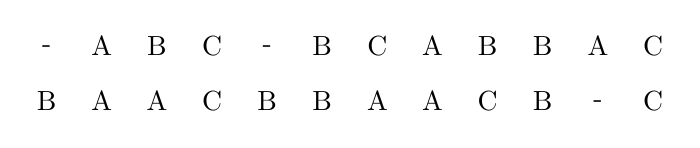
\begin{tikzpicture}[scale=0.7]
\node(t1) at (1, 1) {-};
\node(t2) at (2, 1) {A};
\node(t3) at (3, 1) {B};
\node(t4) at (4, 1) {C};
\node(t5) at (5, 1) {-};
\node(t6) at (6, 1) {B};
\node(t7) at (7, 1) {C};
\node(t8) at (8, 1) {A};
\node(t9) at (9, 1) {B};
\node(t10) at (10, 1) {B};
\node(t11) at (11, 1) {A};
\node(t12) at (12, 1) {C};

\node(l1) at (1, 0) {B};
\node(l2) at (2, 0) {A};
\node(l3) at (3, 0) {A};
\node(l4) at (4, 0) {C};
\node(l5) at (5, 0) {B};
\node(l6) at (6, 0) {B};
\node(l7) at (7, 0) {A};
\node(l8) at (8, 0) {A};
\node(l9) at (9, 0) {C};
\node(l10) at (10, 0) {B};
\node(l11) at (11, 0) {-};
\node(l12) at (12, 0) {C};

\end{tikzpicture}

\textbf{Még egy jópofa sztringes feladat} (egy időben a programozási versenyek kedvence volt)\\
Adott egy $T$ karaktersorozat, keressünk ebben egy leghosszabb olyan karaktersorozatot, amely balról jobbra olvasva ugyanaz, mint jobbról balra olvasva (palindrom)

\sethlcolor{orange}
Pl. T $\longrightarrow$ C {\fcolorbox{blue}{white}{\hl{A}}} D \fcolorbox{blue}{white}{\hl{B}} \hl{C} E \fcolorbox{blue}{white}{\hl{B}} E \fcolorbox{blue}{white}{\hl{A}} B

{\color{blue} Ez egy részsorozat, de nem a leghosszabb.}
{\color{orange} Ez is egy részsorozat, a leghosszabb.}

$T$-ből készítsünk palindromot a legkevesebb karakter törlésével!

Hasonló feladat: $T$-ből készítsünk palindromot a legkevesebb karakter beszúrásával!